% !TEX root=./adl.tex

\section{Modern Transformer Improvements}

% -----------------------------------------------------------------------
\begin{frame}{From GPT-2 to Modern LLMs}

  GPT-2 (2019) established the decoder-only Transformer blueprint. Modern models keep the core design but improve multiple components:

  \vspace{0.5em}
  \begin{center}
  {\small
  \begin{tabular}{lll}
    \toprule
    \textbf{Component} & \textbf{GPT-2} & \textbf{Modern (e.g.\ LLaMA, Gemma)} \\
    \midrule
    Positional encoding & Learned absolute & RoPE (relative) \\
    Normalization       & LayerNorm (pre-norm)  & RMSNorm; Peri-LN + QK-norm \\
    MLP activation      & GELU               & SwiGLU \\
    Attn + MLP          & Sequential         & Sequential (or parallel) \\
    Attention heads      & Multi-Head (MHA)  & GQA; optional gating \\
    KV-cache             & Full (all heads)  & Reduced (GQA, MLA, \ldots) \\
    Biases              & Optional           & Removed entirely \\
    \bottomrule
  \end{tabular}
  }
  \end{center}

  \vspace{0.5em}
  \begin{alertblock}{Key theme}
    None of these changes alter the fundamental architecture.
    Each targets a specific bottleneck -- training stability, inference memory, or compute efficiency -- and the gains compound.
  \end{alertblock}
\end{frame}


% =======================================================================
\subsection{KV-Cache}
% =======================================================================

% -----------------------------------------------------------------------
\begin{frame}{Training vs.\ Inference}

  \begin{columns}[T]
    \begin{column}{0.48\textwidth}
      \textbf{Training (parallel):}
      \begin{itemize}
        \item Feed the full sequence at once
        \item Causal mask ensures each position only sees past tokens
        \item All $T$ next-token losses computed simultaneously
      \end{itemize}

      \vspace{0.3em}
      \begin{center}
      \begin{tikzpicture}[scale=0.80,
          tok/.style={draw=gray!50, rounded corners=2pt, minimum height=0.38cm,
                      inner sep=3pt, font=\scriptsize},
          arr/.style={-{Stealth[length=3pt]}, gray!60, thin},
        ]
        % Input tokens (shifted right by 1 = teacher forcing)
        \node[font=\scriptsize, gray, anchor=east] at (-0.15, 0) {input:};
        \foreach \i/\t in {0/\textlangle s\textrangle, 1/The, 2/cat, 3/sat} {
          \pgfmathsetmacro{\tx}{\i * 1.20}
          \node[tok, fill=xcol] at (\tx, 0) {\t};
        }

        % Transformer block
        \node[draw=gray!50, fill=gray!8, rounded corners=4pt,
              minimum width=5.0cm, minimum height=0.50cm, font=\small]
          at (1.80, 1.00) {Transformer (masked)};

        % Arrows up
        \foreach \i in {0,...,3} {
          \pgfmathsetmacro{\tx}{\i * 1.20}
          \draw[arr] (\tx, 0.22) -- (\tx, 0.74);
        }

        % Output predictions (all in parallel)
        \node[font=\scriptsize, gray, anchor=east] at (-0.15, 2.00) {predict:};
        \foreach \i/\t in {0/The, 1/cat, 2/sat, 3/\textlangle /s\textrangle} {
          \pgfmathsetmacro{\tx}{\i * 1.20}
          \node[tok, fill=zcol] at (\tx, 2.00) {\t};
          \draw[arr] (\tx, 1.26) -- (\tx, 1.78);
        }

        % Loss arrows
        \node[font=\scriptsize, gray] at (1.80, 2.55) {$\mathcal{L} = -\sum_{t=1}^{T} \log p(x_t \mid x_{<t})$};
      \end{tikzpicture}
      \end{center}
    \end{column}
    \begin{column}{0.50\textwidth}
      \textbf{Inference (autoregressive):}
      \begin{itemize}
        \item Generate one token at a time
        \item Append each new token to the context
        \item KV-cache avoids recomputing past keys/values
      \end{itemize}

      \vspace{0.3em}
      \begin{center}
      \begin{tikzpicture}[scale=0.80,
          tok/.style={draw=gray!50, rounded corners=2pt, minimum height=0.38cm,
                      inner sep=3pt, font=\scriptsize},
          arr/.style={-{Stealth[length=3pt]}, gray!60, thin},
        ]
        % Step-by-step generation shown vertically

        % Step 1
        \node[font=\scriptsize, gray, anchor=east] at (-0.30, 2.80) {step 1:};
        \node[tok, fill=xcol] at (0.30, 2.80) {\textlangle s\textrangle};
        \node[font=\scriptsize, gray] at (1.20, 2.80) {$\to$};
        \node[tok, fill=zcol] at (1.90, 2.80) {The};

        % Step 2
        \node[font=\scriptsize, gray, anchor=east] at (-0.30, 2.10) {step 2:};
        \node[tok, fill=xcol] at (0.30, 2.10) {\textlangle s\textrangle};
        \node[tok, fill=xcol] at (1.20, 2.10) {The};
        \node[font=\scriptsize, gray] at (2.00, 2.10) {$\to$};
        \node[tok, fill=zcol] at (2.60, 2.10) {cat};

        % Step 3
        \node[font=\scriptsize, gray, anchor=east] at (-0.30, 1.40) {step 3:};
        \node[tok, fill=xcol] at (0.30, 1.40) {\textlangle s\textrangle};
        \node[tok, fill=xcol] at (1.20, 1.40) {The};
        \node[tok, fill=xcol] at (2.00, 1.40) {cat};
        \node[font=\scriptsize, gray] at (2.80, 1.40) {$\to$};
        \node[tok, fill=zcol] at (3.40, 1.40) {sat};

        % Step 4
        \node[font=\scriptsize, gray, anchor=east] at (-0.30, 0.70) {step 4:};
        \node[tok, fill=xcol] at (0.30, 0.70) {\textlangle s\textrangle};
        \node[tok, fill=xcol] at (1.20, 0.70) {The};
        \node[tok, fill=xcol] at (2.00, 0.70) {cat};
        \node[tok, fill=xcol] at (2.80, 0.70) {sat};
        \node[font=\scriptsize, gray] at (3.55, 0.70) {$\to$};
        \node[tok, fill=zcol] at (4.20, 0.70) {\textlangle /s\textrangle};

        % Annotation
        \node[font=\scriptsize, gray, align=center] at (2.00, 0.00)
          {each step: forward pass $\to$ sample $\to$ append};
      \end{tikzpicture}
      \end{center}
    \end{column}
  \end{columns}
\end{frame}

% -----------------------------------------------------------------------
\begin{frame}{KV-Cache: Avoiding Redundant Computation}

  \begin{columns}[T]
    \begin{column}{0.48\textwidth}
      \textbf{Key insight:} In causal attention, $K$ and $V$ for past positions never change.
      Na\"ive generation recomputes them at every step -- wasteful!

      \vspace{0.3em}
      \textbf{Complexity:}
      \begin{itemize}
        \item \textbf{Prefill} $O(T^2)$: all $T$ tokens attend to each other (full attention matrix).
        \item \textbf{Decode} $O(T)$ per token: only one new $q_t$ attends over cached $K_{1:t}, V_{1:t}$. No recomputation of past keys/values needed.
      \end{itemize}

      \vspace{0.3em}
      \begin{center}
      \begin{tikzpicture}[scale=0.72,
          box/.style={draw=gray!60, rounded corners=2pt,
                      minimum height=0.5cm, font=\tiny, align=center, inner sep=3pt},
          wide/.style={box, minimum width=2.6cm},
          narrow/.style={box, minimum width=2.0cm},
          arr/.style={-{Stealth[length=2.5pt]}, semithick, gray!70},
        ]
        % Top: common entry
        \node[wide, fill=gray!12] (input) at (0, 0) {Receive prompt tokens};

        % Branch point
        \coordinate (split) at (0, -0.55);
        \draw[arr] (input) -- (split);

        % --- Prefill branch (left) ---
        \node[narrow, fill=xcol, font=\tiny\bfseries] (pf) at (-2.1, -1.3) {Prefill};
        \node[narrow, fill=gray!8] (pf1) at (-2.1, -2.2)
          {$Q,K,V$ for all $P$ tokens};
        \node[narrow, fill=kcol!30] (pf2) at (-2.1, -3.1)
          {Store $K,V$ in cache};

        \draw[arr] (split) -| (pf);
        \draw[arr] (pf) -- (pf1);
        \draw[arr] (pf1) -- (pf2);

        % --- Decode branch (right) ---
        \node[narrow, fill=zcol, font=\tiny\bfseries] (dc) at (2.1, -1.3) {Decode};
        \node[narrow, fill=gray!8] (dc1) at (2.1, -2.2)
          {$q_t, k_t, v_t$ for 1 token};
        \node[narrow, fill=orange!20] (dc2) at (2.1, -3.1)
          {Append $k_t, v_t$ to cache};
        \node[narrow, fill=green!15] (dc3) at (2.1, -4.0)
          {$q_t$ attends full cache};
        \node[narrow, fill=zcol] (dc4) at (2.1, -4.8)
          {Sample next token};

        \draw[arr] (split) -| (dc);
        \draw[arr] (dc) -- (dc1);
        \draw[arr] (dc1) -- (dc2);
        \draw[arr] (dc2) -- (dc3);
        \draw[arr] (dc3) -- (dc4);

        % Loop arrow back
        \draw[arr, dashed] (dc4.west) -- +(-0.5,0) |- (dc.west);

        % Connect prefill -> decode
        \draw[arr, densely dotted] (pf2.east) -- node[below, font=\tiny, gray] {once} (dc2.west|-pf2.east);
      \end{tikzpicture}
      \end{center}
    \end{column}
    \begin{column}{0.50\textwidth}
      \begin{center}
      \begin{tikzpicture}[scale=0.82,
          tok/.style={draw=gray!50, rounded corners=2pt, minimum height=0.36cm,
                      minimum width=0.75cm, inner sep=2pt, font=\tiny},
          arr/.style={-{Stealth[length=2.5pt]}, gray!60, thin},
          cachelbl/.style={font=\tiny, gray},
        ]
        % Title
        \node[font=\scriptsize\bfseries, gray] at (2.2, 5.6) {Decode step $t{=}4$};

        % --- Input row ---
        \node[cachelbl, anchor=east] at (-0.15, 4.8) {input:};
        \foreach \i/\t/\c in {0/\textlangle s\textrangle/gray!15, 1/The/gray!15, 2/cat/gray!15, 3/sat/xcol} {
          \pgfmathsetmacro{\tx}{\i * 1.10 + 0.35}
          \node[tok, fill=\c] at (\tx, 4.8) {\t};
        }
        \node[font=\tiny, red!60!black] at (3.85, 4.8) {$\leftarrow$ new};

        % --- Q row: only new token ---
        \node[cachelbl, anchor=east] at (-0.15, 3.8) {$Q$:};
        \foreach \i/\c in {0/white, 1/white, 2/white} {
          \pgfmathsetmacro{\tx}{\i * 1.10 + 0.35}
          \node[tok, draw=none, text=gray!30] at (\tx, 3.8) {--};
        }
        \node[tok, fill=qcol] at (3.65, 3.8) {$q_4$};
        \node[font=\tiny, violet!70] at (4.5, 3.8) {compute};

        % --- K row: cached + new ---
        \node[cachelbl, anchor=east] at (-0.15, 2.8) {$K$:};
        \node[tok, fill=kcol!50] (ck1) at (0.35, 2.8) {$k_1$};
        \node[tok, fill=kcol!50] (ck2) at (1.45, 2.8) {$k_2$};
        \node[tok, fill=kcol!50] (ck3) at (2.55, 2.8) {$k_3$};
        \node[tok, fill=kcol] at (3.65, 2.8) {$k_4$};
        \path let \p1=(ck1.south west), \p2=(ck3.south east) in
          coordinate (kbL) at (\x1, \y1-0.08cm)
          coordinate (kbR) at (\x2, \y1-0.08cm);
        \draw[decorate, decoration={brace, amplitude=3pt, mirror}, orange!60, thick]
          (kbL) -- (kbR)
          node[midway, below=5pt, font=\tiny, orange!80!black] {cached};
        \node[font=\tiny, orange!70] at (4.5, 2.8) {new};

        % --- V row: cached + new ---
        \node[cachelbl, anchor=east] at (-0.15, 1.4) {$V$:};
        \node[tok, fill=vcol!50] (cv1) at (0.35, 1.4) {$v_1$};
        \node[tok, fill=vcol!50] (cv2) at (1.45, 1.4) {$v_2$};
        \node[tok, fill=vcol!50] (cv3) at (2.55, 1.4) {$v_3$};
        \node[tok, fill=vcol] at (3.65, 1.4) {$v_4$};
        \path let \p1=(cv1.south west), \p2=(cv3.south east) in
          coordinate (vbL) at (\x1, \y1-0.08cm)
          coordinate (vbR) at (\x2, \y1-0.08cm);
        \draw[decorate, decoration={brace, amplitude=3pt, mirror}, cyan!50, thick]
          (vbL) -- (vbR)
          node[midway, below=5pt, font=\tiny, cyan!60!black] {cached};
        \node[font=\tiny, cyan!50!black] at (4.5, 1.4) {new};

        % --- Attention computation ---
        \draw[arr, thick] (2.2, 0.4) -- (2.2, -0.1);
        \node[draw=gray!50, fill=green!10, rounded corners=3pt,
              minimum width=3.6cm, minimum height=0.45cm, font=\scriptsize]
          at (2.2, -0.40) {$\text{softmax}\!\bigl(\frac{q_4 K_{1:4}^\top}{\sqrt{d_k}}\bigr) V_{1:4}$};

        % --- Output ---
        \draw[arr, thick] (2.2, -0.65) -- (2.2, -1.05);
        \node[tok, fill=zcol, font=\scriptsize] at (2.2, -1.30) {output $o_4$};
      \end{tikzpicture}
      \end{center}
    \end{column}
  \end{columns}
\end{frame}

% -----------------------------------------------------------------------
\begin{frame}{KV-Cache: Prefill vs.\ Decode}

  \begin{columns}[T]
    \begin{column}{0.48\textwidth}
      \textbf{Prefill} (compute-bound):
      \begin{itemize}
        \item Large matrix multiplies, high arithmetic intensity
        \item Na\"ive cost: $O(T \cdot d)$ projections $+$ $O(T^2 \cdot d)$ attention
      \end{itemize}

      \vspace{0.5em}
      \textbf{Decode} (memory-bound):
      \begin{itemize}
        \item Reading KV-cache dominates; only 1 query vector per step
        \item $O(d)$ projection $+$ $O(t \cdot d)$ attention per step
      \end{itemize}
    \end{column}
    \begin{column}{0.50\textwidth}
      \textbf{Memory:} cache grows as $O(L \cdot h \cdot T \cdot d_k)$

      {\footnotesize ($L$ layers, $h$ heads, $T$ seq.\ length, $d_k$ head dim).}

      \vspace{0.5em}
      \begin{alertblock}{\small Optimizations}
        KV-cache memory can become very large.
        Techniques for reduction: see next slides.
      \end{alertblock}
    \end{column}
  \end{columns}

\end{frame}

% -----------------------------------------------------------------------
\begin{frame}{KV-Cache: The Memory Problem}

  \textbf{Recall:} KV-cache stores $K$ and $V$ for all past tokens, across all layers and heads.

  \vspace{0.3em}
  \textbf{Total KV-cache size:}
  \[
    \text{KV-cache} = 2 \cdot L \cdot h \cdot T \cdot d_k \cdot b
    \quad \text{bytes}
  \]
  {\footnotesize $L$ = layers, $h$ = heads, $T$ = sequence length, $d_k$ = head dim, $b$ = bytes per element.}

  \vspace{0.3em}
  \textbf{Hypothetical example} (LLaMA-2 70B dimensions with MHA, BF16, $T = 4096$):
  \begin{itemize}
    \item $L = 80$, $h = 64$, $d_k = 128$, $b = 2$
    \item KV-cache $= 2 \times 80 \times 64 \times 4096 \times 128 \times 2 \approx 10.7$\,GB \textbf{per sequence}
    \item At $T = 128$k: $\approx 335$\,GB -- larger than the model itself!
    \item Note: LLaMA-2 70B actually uses GQA ($g{=}8$), reducing this by $8\times$.
  \end{itemize}

  \vspace{0.3em}
  \begin{alertblock}{\small Approaches to Reduce KV-Cache}
    \begin{description}[labelwidth=3cm, leftmargin=3.2cm, font=\small]
      \item[Fewer KV heads] MQA, GQA -- share K,V across query heads
      \item[Compress KV] MLA -- low-rank latent compression
      \item[Fewer tokens] Sliding window -- bound the context
      \item[Share across layers] Cross-layer attention
    \end{description}
  \end{alertblock}

\end{frame}

% -----------------------------------------------------------------------
\begin{frame}{Multi-Query Attention (MQA)}

  \textbf{Idea}~\cite{shazeer2019mqattention}: Keep $h$ separate query heads, but use a
  \emph{single shared} key head and value head.

  \vspace{0.3em}
  \begin{columns}[T]
    \begin{column}{0.52\textwidth}
      \textbf{Standard MHA} (per head $i$):
      \[
        Q_i = X W_i^Q,\; K_i = X W_i^K,\; V_i = X W_i^V
      \]
      Each head has its own $W_i^K, W_i^V$.

      \vspace{0.3em}
      \textbf{MQA}:
      \[
        Q_i = X W_i^Q,\; K = X W^K,\; V = X W^V
      \]
      \emph{All} heads share a single $W^K, W^V$ (no subscript $i$).

      \vspace{0.3em}
      \textbf{KV-cache reduction:} $h \times$
      \begin{itemize}
        \item MHA: $2 \cdot h \cdot T \cdot d_k$ per layer
        \item MQA: $2 \cdot 1 \cdot T \cdot d_k$ per layer
      \end{itemize}

      \vspace{0.3em}
      \textbf{Trade-off:} Significant memory savings, but some quality degradation since K,V have reduced capacity.
    \end{column}
    \begin{column}{0.46\textwidth}
      \centering
      \begin{tikzpicture}[scale=0.75,
          headbox/.style={draw, rounded corners=2pt, minimum width=0.7cm,
                          minimum height=0.5cm, font=\tiny, inner sep=1pt},
          kvbox/.style={draw, rounded corners=2pt, minimum width=0.7cm,
                        minimum height=0.5cm, font=\tiny, inner sep=1pt},
          arr/.style={-{Stealth[length=2pt]}, gray!70, thin},
        ]

        % --- MHA ---
        \node[font=\scriptsize\bfseries] at (1.65, 4.6) {MHA};
        \foreach \i in {0,...,3} {
          \pgfmathsetmacro{\xp}{\i * 1.1 + 0.0}
          \node[headbox, fill=qcol] (q\i) at (\xp, 3.8) {$Q_{\the\numexpr\i+1}$};
          \node[kvbox, fill=kcol] (k\i) at (\xp, 2.7) {$K_{\the\numexpr\i+1}$};
          \node[kvbox, fill=vcol] (v\i) at (\xp, 1.7) {$V_{\the\numexpr\i+1}$};
          \draw[arr] (q\i) -- (k\i);
          \draw[arr] (k\i) -- (v\i);
        }

        % --- MQA ---
        \node[font=\scriptsize\bfseries] at (1.65, 0.7) {MQA};
        \foreach \i in {0,...,3} {
          \pgfmathsetmacro{\xp}{\i * 1.1 + 0.0}
          \node[headbox, fill=qcol] (mq\i) at (\xp, 0.0) {$Q_{\the\numexpr\i+1}$};
        }
        \node[kvbox, fill=kcol] (mk) at (1.65, -1.1) {$K$};
        \node[kvbox, fill=vcol] (mv) at (1.65, -2.0) {$V$};
        \foreach \i in {0,...,3} {
          \draw[arr] (mq\i) -- (mk);
        }
        \draw[arr] (mk) -- (mv);
      \end{tikzpicture}
    \end{column}
  \end{columns}

\end{frame}

% -----------------------------------------------------------------------
\begin{frame}{Grouped Query Attention (GQA)}

  \textbf{Idea}~\cite{ainslie2023gqa}: Interpolate between MHA and MQA.
  Divide $h$ query heads into $g$ groups; each group shares one K,V head.

  \vspace{0.3em}
  \begin{columns}[T]
    \begin{column}{0.50\textwidth}
      For group $j$ and query head $i \in \text{group } j$:
      \[
        Q_i = X W_i^Q, \quad K_j = X W_j^K, \quad V_j = X W_j^V
      \]
      \[
        \text{head}_i = \mathrm{softmax}\!\Bigl(\frac{Q_i K_j^\top}{\sqrt{d_k}}\Bigr) V_j
      \]

      \vspace{0.2em}
      \begin{description}[labelwidth=1.4cm, leftmargin=1.6cm, font=\small]
        \item[$g = h$] $\Rightarrow$ MHA (each head has own K,V)
        \item[$g = 1$] $\Rightarrow$ MQA (all heads share K,V)
        \item[$1 < g < h$] $\Rightarrow$ GQA (intermediate)
      \end{description}

      \vspace{0.3em}
      \textbf{KV-cache per layer:} $2 \cdot g \cdot T \cdot d_k$

      \textbf{Reduction vs.\ MHA:} $h / g$
    \end{column}
    \begin{column}{0.48\textwidth}
      \centering
      \begin{tikzpicture}[scale=0.75,
          headbox/.style={draw, rounded corners=2pt, minimum width=0.55cm,
                          minimum height=0.45cm, font=\tiny, inner sep=1pt},
          arr/.style={-{Stealth[length=2pt]}, gray!70, thin},
          grp/.style={draw=gray!40, dashed, rounded corners=3pt, inner sep=3pt},
        ]

        % --- GQA: g=2, h=4 ---
        \node[font=\scriptsize\bfseries] at (1.6, 3.5) {GQA ($h{=}4$, $g{=}2$)};

        % Group 1
        \node[headbox, fill=qcol] (gq1) at (0.0, 2.6) {$Q_1$};
        \node[headbox, fill=qcol] (gq2) at (0.8, 2.6) {$Q_2$};
        \node[headbox, fill=kcol] (gk1) at (0.4, 1.5) {$K_1$};
        \node[headbox, fill=vcol] (gv1) at (0.4, 0.7) {$V_1$};
        \draw[arr] (gq1) -- (gk1);
        \draw[arr] (gq2) -- (gk1);
        \draw[arr] (gk1) -- (gv1);
        \node[grp, fit=(gq1)(gq2)(gv1), label={[font=\tiny, gray]below:group 1}] {};

        % Group 2
        \node[headbox, fill=qcol] (gq3) at (2.4, 2.6) {$Q_3$};
        \node[headbox, fill=qcol] (gq4) at (3.2, 2.6) {$Q_4$};
        \node[headbox, fill=kcol] (gk2) at (2.8, 1.5) {$K_2$};
        \node[headbox, fill=vcol] (gv2) at (2.8, 0.7) {$V_2$};
        \draw[arr] (gq3) -- (gk2);
        \draw[arr] (gq4) -- (gk2);
        \draw[arr] (gk2) -- (gv2);
        \node[grp, fit=(gq3)(gq4)(gv2), label={[font=\tiny, gray]below:group 2}] {};
      \end{tikzpicture}

      \vspace{0.3em}
      {\footnotesize
      \begin{tabular}{lcc}
        \toprule
        \textbf{Model} & $h$ & $g$ \\
        \midrule
        LLaMA-2 70B & 64 & 8 \\
        LLaMA-3 8B & 32 & 8 \\
        Mistral 7B & 32 & 8 \\
        \bottomrule
      \end{tabular}}
    \end{column}
  \end{columns}

\end{frame}

% -----------------------------------------------------------------------
\begin{frame}{GQA: Uptraining from MHA Checkpoints}

  A pretrained MHA model can be converted to GQA without training from scratch~\cite{ainslie2023gqa}.

  \vspace{0.3em}
  \textbf{Recipe:}
  \begin{enumerate}
    \item \textbf{Assign} the $h$ KV heads to $g$ groups (each group has $h/g$ heads).
    \item \textbf{Mean-pool} the KV projection weights within each group:
    \[
      W_j^K = \frac{1}{h/g} \sum_{i \in \text{group } j} W_i^K
      \qquad
      W_j^V = \frac{1}{h/g} \sum_{i \in \text{group } j} W_i^V
    \]
    \item \textbf{Uptrain} with original data for $\sim$5\% of original pretraining compute.
  \end{enumerate}

  \vspace{0.3em}
  \begin{alertblock}{\small Key Results}
    \begin{itemize}
      \item Mean-pool initialization significantly outperforms random initialization.
      \item GQA with $g = 8$ achieves quality close to MHA while approaching MQA inference speed.
      \item LLaMA-2 70B was released with GQA ($g=8$), reducing KV-cache by $8\times$ vs.\ MHA.
    \end{itemize}
  \end{alertblock}

\end{frame}

% -----------------------------------------------------------------------
\begin{frame}{Multi-head Latent Attention (MLA)}

  \textbf{Idea}~\cite{deepseekv2_2024}: Compress the joint KV representation
  into a \emph{low-rank latent vector}
  $\vc^{KV}_t \in \mathbb{R}^{d_c}$ with $d_c \ll n_h \cdot d_h$.
  Only $\vc^{KV}_t$ is cached during inference.

  \vspace{0.3em}
  \begin{columns}[T]
    \begin{column}{0.52\textwidth}
      \begin{itemize}
        \item \textbf{Down-project} (KV compression):
          $\vc^{KV}_t = W^{DKV} \vh_t \in \mathbb{R}^{d_c}$
        \item \textbf{Up-project} to reconstruct K,V:
          $\vk^C_t = W^{UK}\, \vc^{KV}_t$, \;
          $\vv_t = W^{UV}\, \vc^{KV}_t$
        \item \textbf{Queries} (also compressed):
          $\vc^{Q}_t = W^{DQ} \vh_t$, \;
          $\vq^C_t = W^{UQ}\, \vc^{Q}_t$
        \item \textbf{Key insight:} KV information across all heads lies in a low-dimensional subspace.
          Cache the compressed representation, reconstruct on the fly.
      \end{itemize}
    \end{column}
    \begin{column}{0.46\textwidth}
      \centering
      \begin{tikzpicture}[scale=0.80,
          box/.style={draw, rounded corners=2pt, minimum height=0.45cm,
                      font=\tiny, inner sep=2pt, minimum width=1.4cm},
          smallbox/.style={draw, rounded corners=2pt, minimum height=0.40cm,
                      font=\tiny, inner sep=2pt, minimum width=1.0cm},
          arr/.style={-{Stealth[length=2.5pt]}, thick},
        ]

        % h_t
        \node[box, fill=gray!15] (ht) at (-0.8, 4.5) {$\vh_t$};

        % Down-project
        \node[smallbox, fill=green!20] (ckv) at (-0.8, 3.2) {$\vc^{KV}_t$};
        \draw[arr, green!60!black] (ht) -- (ckv) node[midway, left, font=\tiny] {$W^{DKV}$};

        % Up-project K, V
        \node[smallbox, fill=kcol] (kc) at (-1.6, 1.8) {$\vk^C_t$};
        \node[smallbox, fill=vcol] (vt) at (0.0, 1.8) {$\vv_t$};
        \draw[arr, orange!70!black] (ckv) -- (kc) node[midway, left, font=\tiny] {$W^{UK}$};
        \draw[arr, cyan!60!black] (ckv) -- (vt) node[midway, right, font=\tiny] {$W^{UV}$};

        % Cache marker
        \draw[dashed, red!60, thick, rounded corners=3pt]
          ([xshift=-3pt, yshift=-5pt]ckv.south west) rectangle ([xshift=3pt, yshift=5pt]ckv.north east);
        \node[font=\tiny, red!60!black, anchor=west] at (0.0, 3.2) {cached};

        % Dimensions
        \node[font=\tiny, gray, anchor=west] at (0.0, 3.55) {$d_c \ll n_h d_h$};
      \end{tikzpicture}
    \end{column}
  \end{columns}

\end{frame}

% -----------------------------------------------------------------------
\begin{frame}{MLA: Decoupled RoPE}

  \begin{itemize}
    \item \textbf{Problem:} RoPE applies position-dependent rotations $R_t$ to queries and keys:
      $\text{score}_{t,s} = (R_t \vq^C_t)^\top (R_s \vk^C_s)$
    \item Without RoPE, we could absorb the up-projections:
      $(\vq^C_t)^\top \vk^C_s = (\vc^Q_t)^\top \underbrace{(W^{UQ})^\top W^{UK}}_{\text{precomputable}}\, \vc^{KV}_s$
      and \textbf{never materialize full keys}.
      But $R_s$ between $W^{UK}$ and $\vc^{KV}_s$ breaks this.
    \item \textbf{Solution: Decoupled RoPE keys.}
      Add a small separate key carrying positional information:
      \[
        \vk^R_t = R_t\, W^{KR}\, \vh_t \in \mathbb{R}^{d_R}, \qquad
        \vq^R_t = R_t\, W^{QR}\, \vc^Q_t \in \mathbb{R}^{d_R}
      \]
    \item Attention score splits into content + position parts:
      \[
        a_{t,s} = \frac{(\vq^C_t)^\top \vk^C_s + (\vq^R_t)^\top \vk^R_s}{\sqrt{d_h + d_R}}
      \]
    \item \textbf{Cache per token per layer:} $\vc^{KV}_t \in \mathbb{R}^{d_c}$ and $\vk^R_t \in \mathbb{R}^{d_R}$
      $\Rightarrow$ total $d_c + d_R$ elements.
  \end{itemize}

  \vspace{0.3em}
  \begin{exampleblock}{\small DeepSeek-V2 Numbers}
    $n_h{=}128$, $d_h{=}128$, $d_c{=}512$, $d_R{=}64$.
    MHA cache: $2 \times 128 \times 128 = 32{,}768$.
    MLA cache: $512 + 64 = 576$.
    \textbf{Compression: $\mathbf{\sim 57\times}$}.
  \end{exampleblock}

\end{frame}

% -----------------------------------------------------------------------
\begin{frame}{Sliding Window Attention}

  \textbf{Idea}~\cite{jiang2023mistral}: Each token attends only to the $w$ most recent tokens
  instead of the full history.

  \vspace{0.3em}
  \begin{columns}[T]
    \begin{column}{0.52\textwidth}
      Token at position $t$ attends to $\{t{-}w{+}1, \ldots, t\}$:
      \[
        a_{t,s} = \begin{cases}
          \frac{\exp(q_t^\top k_s / \sqrt{d_k})}{\sum_{s'} \exp(\cdot)} & \text{if } s \geq t{-}w{+}1 \\
          0 & \text{otherwise}
        \end{cases}
      \]

      \textbf{Rolling buffer:} cache positions indexed as $t \bmod w$.
      Old entries are overwritten $\Rightarrow$ \textbf{constant memory}.

      \vspace{0.3em}
      \textbf{KV-cache bound per layer:} $2 \cdot h \cdot w \cdot d_k$

      {\footnotesize (independent of total sequence length $T$)}

      \vspace{0.3em}
      \textbf{Effective receptive field:}
      With $L$ layers, information propagates up to $L \times w$ tokens back.
    \end{column}
    \begin{column}{0.46\textwidth}
      \centering
      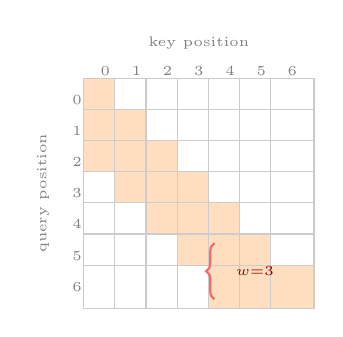
\begin{tikzpicture}[scale=0.72,
          cell/.style={minimum width=0.55cm, minimum height=0.55cm,
                       draw=gray!40, font=\tiny, inner sep=0pt},
        ]
        % Attention matrix
        \def\N{7}
        \def\W{3}
        \foreach \r in {0,...,6} {
          \foreach \c in {0,...,6} {
            \pgfmathtruncatemacro{\causal}{\c <= \r ? 1 : 0}
            \pgfmathtruncatemacro{\inwindow}{\r - \c < \W ? 1 : 0}
            \pgfmathtruncatemacro{\active}{\causal * \inwindow}
            \ifnum\active=1
              \node[cell, fill=orange!25] at (\c*0.55, -\r*0.55) {};
            \else
              \node[cell, fill=white] at (\c*0.55, -\r*0.55) {};
            \fi
          }
        }
        % Labels
        \foreach \i in {0,...,6} {
          \node[font=\tiny, gray] at (\i*0.55, 0.5) {$\i$};
          \node[font=\tiny, gray] at (-0.5, -\i*0.55) {$\i$};
        }
        \node[font=\tiny, gray] at (1.65, 1.0) {key position};
        \node[font=\tiny, gray, rotate=90] at (-1.1, -1.65) {query position};

        % Window annotation
        \draw[decorate, decoration={brace, amplitude=3pt}, red!60, thick]
          (3.5*0.55, -6.4*0.55) -- (3.5*0.55, -4.6*0.55)
          node[midway, right=4pt, font=\tiny, red!60!black] {$w{=}3$};
      \end{tikzpicture}

      \vspace{0.3em}
      {\footnotesize Attention mask for sliding window ($w{=}3$).
      Orange = attended positions.}
    \end{column}
  \end{columns}

  \vspace{0.3em}
  {\footnotesize \textbf{Hybrid:} Some models (Gemma 2, Jamba) alternate sliding window layers
  with full attention layers for bounded cache with some global context.}

\end{frame}

% -----------------------------------------------------------------------
\begin{frame}{Cross-Layer Attention (CLA)}

  \begin{columns}[T]
    \begin{column}{0.50\textwidth}
      \textbf{Idea}~\cite{brandon2024cla}: Adjacent layers \emph{share} the same KV-cache.
      Only every $c$-th layer computes K,V; others reuse.

      \vspace{0.3em}
      For layer $\ell$, anchor layer $a(\ell) = c \cdot \lfloor \ell/c \rfloor$:
      \[
        K^{(\ell)} = K^{(a(\ell))}, \quad V^{(\ell)} = V^{(a(\ell))}
      \]
      Each layer keeps its own $W^Q$.

      \vspace{0.3em}
      \begin{itemize}
        \item \textbf{Reduction:} $c\times$ less KV-cache (across layers).
        \item CLA is \emph{orthogonal} to GQA/MQA -- combine for multiplicative savings.
      \end{itemize}
    \end{column}
    \begin{column}{0.48\textwidth}
      \centering
      \begin{tikzpicture}[scale=0.62,
          layer/.style={draw=gray!60, rounded corners=2pt, minimum width=1.0cm,
                        minimum height=0.4cm, font=\tiny, inner sep=2pt},
          kv/.style={draw, rounded corners=2pt, minimum width=0.7cm,
                     minimum height=0.35cm, font=\tiny, inner sep=1pt},
          arr/.style={-{Stealth[length=2pt]}, gray!60, thin},
          share/.style={-{Stealth[length=2pt]}, red!60, semithick, dashed},
        ]
        \def\cx{0}  % shared x center for both diagrams

        % --- Standard (top) ---
        \node[font=\tiny\bfseries, gray] at (\cx, 5.6) {Standard};
        \foreach \i/\lbl in {0/1, 1/2, 2/3, 3/4} {
          \pgfmathsetmacro{\yy}{4.9 - \i * 0.9}
          \node[layer, fill=gray!10] (sL\i) at (\cx, \yy) {Layer \lbl};
          \node[kv, fill=kcol!50, anchor=east] (sK\i) at (\cx-1.5, \yy) {$K^{(\lbl)}$};
          \node[kv, fill=vcol!50, anchor=west] (sV\i) at (\cx+1.5, \yy) {$V^{(\lbl)}$};
          \draw[arr] (sK\i) -- (sL\i);
          \draw[arr] (sV\i) -- (sL\i);
        }
        \foreach \i/\j in {0/1, 1/2, 2/3} {
          \draw[arr] (sL\i) -- (sL\j);
        }

        % --- CLA c=2 (bottom) ---
        \node[font=\tiny\bfseries, gray] at (\cx, 1.3) {CLA ($c{=}2$)};
        \foreach \i/\lbl in {0/1, 1/2, 2/3, 3/4} {
          \pgfmathsetmacro{\yy}{0.6 - \i * 0.9}
          \node[layer, fill=gray!10] (cL\i) at (\cx, \yy) {Layer \lbl};
        }
        \foreach \i/\j in {0/1, 1/2, 2/3} {
          \draw[arr] (cL\i) -- (cL\j);
        }

        % KV for anchor layers (1 and 3)
        \node[kv, fill=kcol, anchor=east] (cK0) at (\cx-1.5, 0.6) {$K^{(1)}$};
        \node[kv, fill=vcol, anchor=west] (cV0) at (\cx+1.5, 0.6) {$V^{(1)}$};
        \draw[arr] (cK0) -- (cL0);
        \draw[arr] (cV0) -- (cL0);

        \node[kv, fill=kcol, anchor=east] (cK2) at (\cx-1.5, -1.2) {$K^{(3)}$};
        \node[kv, fill=vcol, anchor=west] (cV2) at (\cx+1.5, -1.2) {$V^{(3)}$};
        \draw[arr] (cK2) -- (cL2);
        \draw[arr] (cV2) -- (cL2);

        % Shared arrows
        \draw[share] (cK0.south) |- (cL1.west);
        \draw[share] (cV0.south) |- (cL1.east);
        \draw[share] (cK2.south) |- (cL3.west);
        \draw[share] (cV2.south) |- (cL3.east);

        % Labels
        \node[font=\tiny, red!60!black] at (\cx-2.2, -0.5) {shared};
        \node[font=\tiny, red!60!black] at (\cx-2.2, -2.3) {shared};
      \end{tikzpicture}
    \end{column}
  \end{columns}

\end{frame}

% -----------------------------------------------------------------------
\begin{frame}{KV-Cache Reduction: Summary}

  \begin{center}
  {\small
  \begin{tabular}{llcc}
    \toprule
    \textbf{Method} & \textbf{Core idea} & \textbf{Cache per layer per token} & \textbf{vs.\ MHA} \\
    \midrule
    MHA & Separate K,V per head & $2\, h\, d_k$ & $1\times$ \\
    MQA & Single shared K,V & $2\, d_k$ & $1/h$ \\
    GQA-$g$ & $g$ groups share K,V & $2\, g\, d_k$ & $g/h$ \\
    MLA & Low-rank KV compression & $d_c + d_R$ & $\sim 1/57\times$ \\
    Sliding window & Attend to last $w$ tokens & $2\, h\, d_k$ (capped at $w$) & $w / T$ \\
    CLA (factor $c$) & Share KV across $c$ layers & $2\, h\, d_k / c$ (amortized) & $1/c$ \\
    \bottomrule
  \end{tabular}
  }
  \end{center}

  \vspace{0.3em}
  \textbf{Key points:}
  \begin{itemize}
    \item These techniques are largely \textbf{orthogonal and composable}.
    \item GQA is the current standard (LLaMA-2/3, Mistral, Gemma).
    \item MLA (DeepSeek-V2/V3) achieves the strongest compression while retaining multi-head expressiveness.
    \item In practice, models combine multiple techniques:
      e.g.\ Mistral = GQA + sliding window; DeepSeek-V3 = MLA + other efficiencies.
  \end{itemize}

\end{frame}

\subsection{RoPE}

% !TEX root=./adl.tex

% -----------------------------------------------------------------------
\begin{frame}{Limitations of Absolute Positional Encodings}

  Recall: sinusoidal or learned PE are \textbf{added} to token embeddings before attention.

  \vspace{0.5em}
  \textbf{Problems:}
  \begin{itemize}
    \item Attention scores depend on \emph{absolute} positions, not relative distance
    \item Sinusoidal PE: dot product $\text{PE}(m)^\top \text{PE}(n)$ depends on both $m$ and $n$, not just $m - n$
    \item Learned PE: cannot generalize beyond the maximum training length
    \item Adding PE to content embeddings mixes positional and semantic information
  \end{itemize}

  \vspace{0.5em}
  \begin{alertblock}{Desiderata}
    \begin{itemize}
      \item Attention score $\vq_m^\top \vk_n$ should depend on relative distance $m - n$
      \item Positional information should be \emph{injected into} Q and K, not added to content
      \item No learned parameters
    \end{itemize}
  \end{alertblock}

\end{frame}

% -----------------------------------------------------------------------
\begin{frame}{RoPE: Core Idea~\cite{su2024roformer}}

  \textbf{Key insight:} Encode position by \emph{rotating} query and key vectors.

  \vspace{0.3em}
  \begin{columns}[T]
    \begin{column}{0.52\textwidth}
      \begin{itemize}
        \item 2D subspace, position $m$, rotate by $m\theta$:
          \[
            R(m\theta) = \begin{pmatrix} \cos m\theta & -\sin m\theta \\ \sin m\theta & \cos m\theta \end{pmatrix}
          \]
          \vspace{-0.8em}
        \item Query and key at positions $m$, $n$:
          \[
            \tilde{\vq}_m = R(m\theta)\,\vq_m, \quad \tilde{\vk}_n = R(n\theta)\,\vk_n
          \]
          \vspace{-0.8em}
        \item Dot product:
          \vspace{-0.3em}
          \begin{align*}
            \tilde{\vq}_m^\top \tilde{\vk}_n &= \vq_m^\top R(m\theta)^\top R(n\theta)\,\vk_n \\
            &= \vq_m^\top R\bigl((n{-}m)\theta\bigr)\,\vk_n
          \end{align*}
          \vspace{-0.8em}
        \item Since $R(\alpha)^\top = R(-\alpha)$ (orthogonal):
          \vspace{-0.3em}
          \begin{align*}
            R(\alpha)^\top R(\beta) &= R(-\alpha)\,R(\beta) = R(\beta - \alpha)
          \end{align*}
      \end{itemize}
    \end{column}

    \begin{column}{0.45\textwidth}
      \begin{center}
      \begin{tikzpicture}[scale=0.92]
        % Axes
        \draw[-{Stealth[length=3pt]}, gray!50] (-2.3,0) -- (2.5,0);
        \draw[-{Stealth[length=3pt]}, gray!50] (0,-0.6) -- (0,2.5);

        % Unit circle (upper half)
        \draw[gray!25, dashed] (0,0) circle(2.0);

        % --- Angle definitions (chosen to avoid overlaps) ---
        \pgfmathsetmacro{\qang}{15}      % original q direction
        \pgfmathsetmacro{\mtheta}{55}    % q rotation = m*theta
        \pgfmathsetmacro{\qrot}{\qang + \mtheta}  % = 70

        \pgfmathsetmacro{\kang}{-40}     % original k direction
        \pgfmathsetmacro{\ntheta}{25}    % k rotation = n*theta
        \pgfmathsetmacro{\krot}{\kang + \ntheta}  % = -15

        % --- Original q (dashed) ---
        \draw[-{Stealth[length=4pt]}, blue!30, thick, dashed] (0,0) --
          ({2.0*cos(\qang)}, {2.0*sin(\qang)});
        \node[font=\tiny, blue!30, anchor=west] at
          ({2.05*cos(\qang)}, {2.0*sin(\qang)}) {$\vq_m$};

        % --- Rotated q (solid) ---
        \draw[-{Stealth[length=4pt]}, blue!70!black, thick] (0,0) --
          ({2.0*cos(\qrot)}, {2.0*sin(\qrot)});
        \node[font=\tiny, blue!70!black, anchor=south west] at
          ({2.0*cos(\qrot)+0.02}, {2.0*sin(\qrot)+0.02}) {$\tilde{\vq}_m$};

        % Arc for q rotation (inner, r=0.85)
        \draw[-{Stealth[length=2pt]}, blue!50, thick]
          ({0.85*cos(\qang)}, {0.85*sin(\qang)})
          arc[start angle=\qang, end angle=\qrot, radius=0.85];
        \node[font=\tiny, blue!50, anchor=south] at
          ({1.1*cos((\qang+\qrot)/2)}, {1.1*sin((\qang+\qrot)/2)}) {$m\theta$};

        % --- Original k (dashed) ---
        \draw[-{Stealth[length=4pt]}, orange!40, thick, dashed] (0,0) --
          ({2.0*cos(\kang)}, {2.0*sin(\kang)});
        \node[font=\tiny, orange!40, anchor=north] at
          ({2.0*cos(\kang)}, {2.0*sin(\kang)-0.1}) {$\vk_n$};

        % --- Rotated k (solid) ---
        \draw[-{Stealth[length=4pt]}, orange!70!black, thick] (0,0) --
          ({2.0*cos(\krot)}, {2.0*sin(\krot)});
        \node[font=\tiny, orange!70!black, anchor=north west] at
          ({2.0*cos(\krot)+0.05}, {2.0*sin(\krot)-0.08}) {$\tilde{\vk}_n$};

        % Arc for k rotation (innermost, r=0.6)
        \draw[-{Stealth[length=2pt]}, orange!50, thick]
          ({0.6*cos(\kang)}, {0.6*sin(\kang)})
          arc[start angle=\kang, end angle=\krot, radius=0.6];
        \node[font=\tiny, orange!50, anchor=west] at
          ({0.8*cos((\kang+\krot)/2)}, {0.8*sin((\kang+\krot)/2)}) {$n\theta$};

        % --- Angle between rotated vectors (outermost, r=1.5) ---
        \draw[{Stealth[length=2pt]}-{Stealth[length=2pt]}, red!60!black, thick]
          ({1.5*cos(\krot)}, {1.5*sin(\krot)})
          arc[start angle=\krot, end angle=\qrot, radius=1.5];
        \node[font=\scriptsize, red!60!black, anchor=south west] at
          ({1.7*cos((\qrot+\krot)/2)}, {1.7*sin((\qrot+\krot)/2)}) {$(n{-}m)\theta$};

      \end{tikzpicture}
      \end{center}
    \end{column}
  \end{columns}

  \vspace{0.3em}
  \begin{block}{Result}
    The attention score depends only on relative position $n - m$ and the content vectors.
  \end{block}

\end{frame}

% -----------------------------------------------------------------------
\begin{frame}{RoPE: Complex Number View}

  Equivalently, represent each dimension pair $(x_{2i}, x_{2i+1})$ as a complex number:
  \[
    z_i = x_{2i} + j\, x_{2i+1} \in \mathbb{C}
  \]

  RoPE at position $m$: multiply by a unit complex number
  \[
    \tilde{z}_i = z_i \cdot e^{j\, m \theta_i}
  \]

  \vspace{0.3em}
  The dot product between rotated queries and keys becomes:
  \[
    \operatorname{Re}\!\left(\tilde{z}_i^{(q)} \cdot \overline{\tilde{z}_i^{(k)}}\right) = \operatorname{Re}\!\left(z_i^{(q)} \cdot \overline{z_i^{(k)}} \cdot e^{j\,(m-n)\theta_i}\right)
  \]

  \vspace{0.3em}
  \begin{block}{Implementation in practice}
    \begin{itemize}
      \item Reshape Q, K into pairs: $(d/2)$ complex numbers
      \item Precompute $e^{j\, m \theta_i}$ for all positions $m$ and frequencies $i$
      \item Element-wise complex multiply (or equivalent real-valued formula)
    \end{itemize}
  \end{block}

\end{frame}

% -----------------------------------------------------------------------
\begin{frame}{RoPE: Full Rotation Matrix}

  For head dimension $d$, apply different rotation frequencies $\theta_i$ to each pair:
  \[
    \theta_i = \frac{1}{b^{2i/d}}, \quad i = 0, 1, \ldots, d/2 - 1
  \]
  where $b = 10{,}000$ is the base (same convention as sinusoidal PE).

  \vspace{0.3em}
  The full rotation matrix at position $m$ is block-diagonal:
  \[
    R_m = \begin{pmatrix}
      R(m\theta_0) & & \\
      & R(m\theta_1) & \\
      & & \ddots \\
      & & & R(m\theta_{d/2-1})
    \end{pmatrix}
  \]

  \vspace{0.3em}
  \begin{description}[labelwidth=\widthof{\bfseries High dimensions:~~}, leftmargin=!]
    \item[Low dimensions:] large $\theta_i$ $\Rightarrow$ fast rotation $\Rightarrow$ captures fine-grained local position
    \item[High dimensions:] small $\theta_i$ $\Rightarrow$ slow rotation $\Rightarrow$ captures long-range position
  \end{description}

  Analogous to the frequency spectrum in sinusoidal PE.

\end{frame}

% -----------------------------------------------------------------------
\begin{frame}{RoPE: Visualization}

  \begin{center}
  \begin{tikzpicture}[scale=0.85]

    % --- Left: 2D rotation diagram ---
    \begin{scope}[shift={(-3.2, 0)}]
      \draw[-{Stealth[length=3pt]}, gray!60] (-0.3,0) -- (2.5,0) node[right, font=\tiny, gray] {$x_{2i}$};
      \draw[-{Stealth[length=3pt]}, gray!60] (0,-0.3) -- (0,2.5) node[above, font=\tiny, gray] {$x_{2i+1}$};

      % Original vector
      \draw[-{Stealth[length=4pt]}, thick, blue!70!black] (0,0) -- (2.0, 0.73);
      \node[font=\scriptsize, blue!70!black, anchor=south west] at (2.0, 0.73) {$\vq_m$};

      % Rotated vector
      \draw[-{Stealth[length=4pt]}, thick, red!70!black] (0,0) -- (1.1, 1.82);
      \node[font=\scriptsize, red!70!black, anchor=south east] at (1.0, 1.9) {$\tilde{\vq}_m$};

      % Arc for angle
      \draw[-{Stealth[length=2.5pt]}, blue!50, thick] (1.36, 0.50) arc[start angle=20, end angle=59, radius=1.45];
      \node[font=\scriptsize, blue!50] at (1.55, 1.25) {$m\theta_i$};

      % Dashed circle
      \draw[gray!30, dashed] (0,0) circle(2.13);

      \node[font=\scriptsize, anchor=north] at (1.1, -0.4) {Rotation in pair $(2i, 2i{+}1)$};
    \end{scope}

    % --- Right: frequency spectrum ---
    \begin{scope}[shift={(1.8, -0.3)}]
      \node[font=\scriptsize, anchor=south] at (1.6, 2.5) {Rotation speed per dimension pair};

      \foreach \i/\speed/\col in {0/fast/red!70, 1/\phantom{x}/red!50, 2/\phantom{x}/orange!60, 3/\phantom{x}/yellow!70!orange, 4/\phantom{x}/green!50, 5/\phantom{x}/teal!50, 6/\phantom{x}/blue!40, 7/slow/blue!70} {
        \pgfmathsetmacro{\bw}{0.35}
        \pgfmathsetmacro{\bx}{\i * 0.43}
        \pgfmathsetmacro{\bh}{2.2 - \i * 0.25}
        \fill[\col] (\bx, 0) rectangle (\bx + \bw, \bh);
        \draw[gray!50, thin] (\bx, 0) rectangle (\bx + \bw, \bh);
        \node[font=\tiny, gray] at (\bx + \bw/2, -0.2) {$\i$};
      }

      \node[font=\tiny, red!70!black, anchor=west] at (3.7, 1.9) {local};
      \node[font=\tiny, blue!70!black, anchor=west] at (3.7, 0.5) {global};
      \draw[-{Stealth[length=2pt]}, gray!50, thin] (3.85, 1.7) -- (3.85, 0.7);

      \node[font=\tiny, gray] at (1.6, -0.4) {dimension pair index $i$};
    \end{scope}

  \end{tikzpicture}
  \end{center}

  \vspace{-0.5em}
  \begin{itemize}
    \item Each dimension pair is rotated independently at its own frequency
    \item Low-index pairs rotate fast (local patterns), high-index pairs rotate slowly (global patterns)
    \item Applied to Q and K \textbf{after} projection, \textbf{before} dot product
  \end{itemize}

\end{frame}

% -----------------------------------------------------------------------
\begin{frame}{RoPE: Properties}

  \begin{columns}[T]
    \begin{column}{0.52\textwidth}
      \begin{description}[labelwidth=\widthof{\bfseries No learned params:~~}, leftmargin=!]
        \item[Relative PE:] $\tilde{\vq}_m^\top \tilde{\vk}_n$ depends on $\vq_m$, $\vk_n$, and $m {-} n$ only
        \item[No learned params:] Fully determined by base $b$ and head dim $d$
        \item[Norm-preserving:] $\|R_m \vq\| = \|\vq\|$ (orthogonal)
        \item[Long-range decay:] As $|m{-}n|$ grows, rotating phases cancel $\Rightarrow$ inner product decays
        \item[Flexible:] Per-head, works with MHA, GQA, MQA
      \end{description}

      \vspace{0.3em}
      \begin{block}{Adoption}
        Used by LLaMA, Mistral, Qwen, Gemma, DeepSeek, and most modern open-weight LLMs.
      \end{block}
    \end{column}

    \begin{column}{0.46\textwidth}
      \textbf{Long-range decay} for unit vectors $\vq = \vk$:
      \vspace{-0.3em}
      \[
        \tilde{\vq}_m^\top \tilde{\vk}_n = \sum_{i=0}^{d/2-1} \cos\bigl((m{-}n)\,\theta_i\bigr)
      \]
      \vspace{-0.5em}

      \begin{center}
      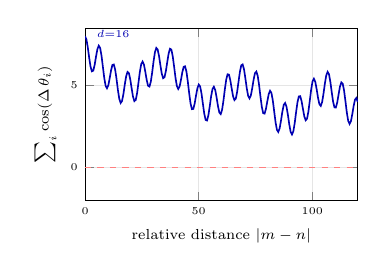
\begin{tikzpicture}[scale=0.75]
        \begin{axis}[
          width=6.2cm, height=4.5cm,
          xlabel={relative distance $|m - n|$},
          ylabel={$\sum_i \cos(\Delta\, \theta_i)$},
          xlabel style={font=\scriptsize},
          ylabel style={font=\scriptsize},
          tick label style={font=\tiny},
          xmin=0, xmax=120,
          ymin=-2, ymax=8.5,
          domain=0:120,
          samples=200,
          grid=major,
          grid style={gray!20},
          every axis plot/.append style={thick},
        ]
          % Sum of cos(delta * theta_i) for d=16 (8 pairs), base=10000
          % theta_i = 1/10000^(2i/16) for i=0..7
          \addplot[blue!70!black, thick] {
            cos(deg(x / 1.0))
            + cos(deg(x / 5.623))
            + cos(deg(x / 31.62))
            + cos(deg(x / 177.8))
            + cos(deg(x / 1000.0))
            + cos(deg(x / 5623.0))
            + cos(deg(x / 31623.0))
            + cos(deg(x / 100000.0))
          };

          % Reference line
          \draw[red!50, dashed, thin] (axis cs:0, 0) -- (axis cs:120, 0);

          % Annotations
          \node[font=\tiny, blue!70!black, anchor=south west] at (axis cs:2, 7.5) {$d{=}16$};
        \end{axis}
      \end{tikzpicture}
      \end{center}
      \vspace{-0.5em}
      {\scriptsize High-freq pairs oscillate and cancel; low-freq pairs decay slowly. Peak at $\Delta{=}0$ (all cosines $= 1$).}
    \end{column}
  \end{columns}

\end{frame}

% -----------------------------------------------------------------------
\begin{frame}{RoPE: Why Long-Range Decay?}

  Expand $\langle R_m \vq, R_n \vk\rangle$ pair by pair using $\cos(m\theta_i)\cos(n\theta_i) + \sin(m\theta_i)\sin(n\theta_i) = \cos(\Delta\theta_i)$, $\Delta = m-n$:
  \[
    \text{score}(m,n) = \sum_{i=0}^{d/2-1} a_i \cos(\Delta\,\theta_i) + b_i \sin(\Delta\,\theta_i)
  \]
  with, on each pair $(2i, 2i{+}1)$,
  \(
    a_i = q_{2i}k_{2i} + q_{2i+1}k_{2i+1}
  \)
  (unrotated dot product) and
  \(
    b_i = q_{2i+1}k_{2i} - q_{2i}k_{2i+1}
  \)
  (2D cross-product). Both are \textbf{content-only}; positions enter only through $\theta_i = \text{base}^{-2i/d}$.

  \vspace{0.3em}
  \begin{columns}[T]
    \begin{column}{0.55\textwidth}
      \textbf{$\Delta = 0$:} $\cos(0){=}1$, $\sin(0){=}0$ $\Rightarrow$ score $= \vq^\top \vk$ (full signal).

      \vspace{0.3em}
      \textbf{Growing $|\Delta|$:} pairs oscillate at different $\theta_i$; phases spread and \textbf{destructively interfere}:
      \begin{itemize}
        \item Small $|\Delta|$: high-freq pairs cancel; low-freq still coherent.
        \item Large $|\Delta|$: nearly all pairs incoherent; score near zero.
      \end{itemize}

      \vspace{0.3em}
      \textbf{Riemann-Lebesgue effect:} a sum of oscillators at spread-out frequencies vanishes as the phase shift grows.
    \end{column}
    \begin{column}{0.43\textwidth}
      \centering
      {\small\textbf{Phasor view} at large $|\Delta|$:}

      \begin{tikzpicture}[scale=0.45]
        % Unit circle
        \draw[gray!30] (0,0) circle(1.8);
        \draw[-{Stealth[length=2pt]}, gray!40] (-2.0,0) -- (2.0,0);
        \draw[-{Stealth[length=2pt]}, gray!40] (0,-2.0) -- (0,2.0);

        % Phasors at different angles (representing e^{j*Delta*theta_i} for various i)
        \foreach \ang/\col in {15/red!70, 72/orange!70, 145/yellow!70!black, 198/green!60!black, 253/teal!70, 290/blue!60, 340/violet!60, 50/red!40} {
          \draw[-{Stealth[length=2.5pt]}, \col, thick] (0,0) -- ({1.8*cos(\ang)},{1.8*sin(\ang)});
        }

        % Sum vector (small, near origin)
        \draw[-{Stealth[length=3pt]}, black, very thick] (0,0) -- (0.3, 0.15);
        \node[font=\tiny, anchor=west] at (0.35, 0.15) {$\sum$};

        \node[font=\tiny, gray, anchor=north] at (0, -2.0) {Phases spread $\Rightarrow$ sum $\approx 0$};
      \end{tikzpicture}

      {\small\textbf{At $\Delta = 0$} all phasors aligned:}

      \begin{tikzpicture}[scale=0.45]
        \draw[gray!30] (0,0) circle(1.8);
        \draw[-{Stealth[length=2pt]}, gray!40] (-2.0,0) -- (2.0,0);
        \draw[-{Stealth[length=2pt]}, gray!40] (0,-2.0) -- (0,2.0);

        % All phasors aligned to the right
        \foreach \i in {1,...,8} {
          \pgfmathsetmacro{\yoff}{(\i - 4.5) * 0.04}
          \draw[-{Stealth[length=2.5pt]}, blue!60, thick] (0,\yoff) -- (1.8,\yoff);
        }

        \draw[-{Stealth[length=3pt]}, black, very thick] (0,0) -- (1.8, 0);
        \node[font=\tiny, anchor=west] at (1.85, 0) {$\sum$};

        \node[font=\tiny, gray, anchor=north] at (0, -2.0) {All aligned $\Rightarrow$ max score};
      \end{tikzpicture}
    \end{column}
  \end{columns}
\end{frame}

% -----------------------------------------------------------------------
\begin{frame}{The Extrapolation Problem}

  RoPE is trained on sequences up to length $L_{\text{train}}$ (e.g.\ 4096 tokens).

  \vspace{0.3em}
  \textbf{At inference}, we want to handle $L_{\text{test}} \gg L_{\text{train}}$.

  \vspace{0.5em}
  \textbf{What goes wrong:}
  \begin{itemize}
    \item Positions $m > L_{\text{train}}$ produce rotation angles $m\theta_i$ never seen during training
    \item Attention logits become unpredictable for out-of-distribution positions
    \item Performance degrades sharply beyond training length
  \end{itemize}

  \vspace{0.5em}
  \textbf{Approaches:}
  \begin{description}[labelwidth=\widthof{\bfseries NTK-aware interpolation:~~}, leftmargin=!]
    \item[Position interpolation:] Scale positions: $m \to m \cdot \frac{L_{\text{train}}}{L_{\text{test}}}$~\cite{chen2023extending}. \\
      All angles stay in $[0, L_{\text{train}} \cdot \theta_i]$. Requires fine-tuning.
    \item[NTK-aware interpolation:] Scale the base $b$ instead of positions~\cite{bloc97_2023ntk}.
      Changes frequencies non-uniformly. Can work without fine-tuning.
    \item[YaRN:] Combines NTK-aware interpolation with attention scaling~\cite{peng2023yarn}.
  \end{description}

\end{frame}

% -----------------------------------------------------------------------
\begin{frame}{Position Interpolation vs.\ Extrapolation}

  Let $s = L_{\text{test}} / L_{\text{train}}$ be the scaling factor.

  \vspace{0.3em}
  \begin{columns}[T]
    \begin{column}{0.48\textwidth}
      \textbf{Extrapolation} (naive):
      \begin{itemize}
        \item Use original $\theta_i$ at all positions
        \item Positions $> L_{\text{train}}$: angles unseen during training
        \item High-frequency pairs: multiple full extra rotations
      \end{itemize}

      \vspace{0.3em}
      \begin{center}
      \begin{tikzpicture}[scale=0.65]
        % Axis
        \draw[-{Stealth[length=3pt]}, gray!60] (0,0) -- (5.5,0) node[right, font=\tiny] {position $m$};
        \draw[-{Stealth[length=3pt]}, gray!60] (0,0) -- (0,3.2) node[above, font=\tiny] {angle $m\theta_i$};

        % Training region
        \fill[green!15] (0,0) rectangle (2.5, 3.0);
        \node[font=\tiny, green!50!black] at (1.25, 2.7) {train};

        % Extrapolation region
        \fill[red!10] (2.5,0) rectangle (5.0, 3.0);
        \node[font=\tiny, red!50!black] at (3.75, 2.7) {unseen};

        % Line
        \draw[thick, blue!70] (0,0) -- (5.0, 3.0);
        \draw[dashed, gray] (2.5, 0) -- (2.5, 3.0);
      \end{tikzpicture}
      \end{center}
    \end{column}

    \begin{column}{0.48\textwidth}
      \textbf{Position Interpolation}:
      \begin{itemize}
        \item Scale: $m \to m/s$
        \item All angles map into training range
        \item Tokens are ``squeezed'' closer together
        \item Fine-tuning needed: model must adapt to denser positions
      \end{itemize}

      \vspace{0.3em}
      \begin{center}
      \begin{tikzpicture}[scale=0.65]
        % Axis
        \draw[-{Stealth[length=3pt]}, gray!60] (0,0) -- (5.5,0) node[right, font=\tiny] {position $m$};
        \draw[-{Stealth[length=3pt]}, gray!60] (0,0) -- (0,3.2) node[above, font=\tiny] {angle $m\theta_i / s$};

        % Training region
        \fill[green!15] (0,0) rectangle (5.0, 3.0);
        \node[font=\tiny, green!50!black] at (2.5, 2.7) {interpolated};

        % Line (shallower slope)
        \draw[thick, orange!70!black] (0,0) -- (5.0, 1.5);

        % Original line (dashed)
        \draw[dashed, blue!40] (0,0) -- (2.5, 1.5);
        \node[font=\tiny, blue!40, anchor=west] at (2.5, 1.7) {original};
      \end{tikzpicture}
      \end{center}
    \end{column}
  \end{columns}

\end{frame}

% -----------------------------------------------------------------------
\begin{frame}{NTK-aware Interpolation}

  \begin{description}[labelwidth=\widthof{\bfseries head dim $d$:~~}, leftmargin=!, font=\small]
    \item[scale $s$:] extension ratio $L_{\text{test}}/L_{\text{train}}$.
    \item[head dim $d$:] $d/2$ rotation pairs $i = 0,\ldots,\tfrac{d}{2}{-}1$ with frequencies $\theta_i = b^{-2i/d}$ and wavelengths $\lambda_i = 2\pi/\theta_i$.
  \end{description}

  \vspace{0.4em}
  \begin{columns}[T]
    \begin{column}{0.40\textwidth}
      \textbf{NTK-aware~\cite{bloc97_2023ntk}.} Scale the base, not positions:
      \[
        b' = b \cdot s^{\,d/(d-2)}.
      \]
      The exponent $\tfrac{d}{d-2}$ makes
      \begin{itemize}
        \item $\theta_0' = \theta_0$ (high freq kept),
        \item $\theta_{\tfrac{d}{2}-1}' = \theta_{\tfrac{d}{2}-1}/s$ (low freq fully interpolated).
      \end{itemize}

      \vspace{0.3em}
      Wavelengths shorter than $L_{\text{train}}$ stay; longer ones are stretched. Works without fine-tuning for $2$--$4\times$ extensions.
    \end{column}
    \begin{column}{0.58\textwidth}
      \centering
      \begin{tikzpicture}[scale=0.82,
          wbar/.style={line width=2.6pt, line cap=round},
          lbl/.style={font=\tiny},
        ]
        % Background regions: train, extension, beyond L_test
        \fill[green!10]  (0,   -0.1) rectangle (2.4, 4.7);
        \fill[orange!10] (2.4, -0.1) rectangle (4.8, 4.7);
        \fill[red!7]     (4.8, -0.1) rectangle (7.6, 4.7);

        % --- bars (drawn before dashed lines so the lines stay visible on top) ---
        % small i: tiny wavelength, NTK unchanged
        \draw[wbar, blue!70]         (0, 4.2)  -- (0.18, 4.2);
        \draw[wbar, orange!80!black] (0, 3.95) -- (0.18, 3.95);
        \node[lbl, anchor=west] at (0.4, 4.07) {small $i$ (high freq): unchanged};

        % medium-small i
        \draw[wbar, blue!70]         (0, 3.1)  -- (1.0, 3.1);
        \draw[wbar, orange!80!black] (0, 2.85) -- (1.3, 2.85);

        % medium i: near L_train, NTK crosses L_train
        \draw[wbar, blue!70]         (0, 2.0)  -- (2.0, 2.0);
        \draw[wbar, orange!80!black] (0, 1.75) -- (3.5, 1.75);

        % large i: long wavelength, heavy stretch
        \draw[wbar, blue!70]         (0, 0.85) -- (3.2, 0.85);
        \draw[wbar, orange!80!black] (0, 0.55) -- (6.6, 0.55);
        \node[lbl, anchor=west, orange!80!black] at (6.7, 0.55) {$\approx s\,\lambda_i$};
        \node[lbl, anchor=west] at (0.05, 0.25) {large $i$ (low freq): stretched};

        % Boundary markers (on top of bars)
        \draw[green!50!black, thick, densely dashed] (2.4, -0.1) -- (2.4, 4.7);
        \draw[red!50!black,   thick, densely dashed] (4.8, -0.1) -- (4.8, 4.7);
        \node[lbl, green!50!black, anchor=south] at (2.4, 4.7) {$L_{\text{train}}$};
        \node[lbl, red!50!black,   anchor=south] at (4.8, 4.7) {$L_{\text{test}}$};

        % Position axis (drawn last so it sits above fills)
        \draw[gray!60, -{Stealth[length=2.5pt]}] (-0.05, -0.1) -- (7.7, -0.1)
          node[right, lbl, gray] {position};

        % Side label
        \node[lbl, gray, rotate=90] at (-0.4, 2.5) {wavelength $\lambda_i$};

        % Legend
        \draw[wbar, blue!70]         (0.0, -0.75) -- (0.3, -0.75);
        \node[lbl, anchor=west] at (0.35, -0.75) {original $\lambda_i$};
        \draw[wbar, orange!80!black] (2.0, -0.75) -- (2.3, -0.75);
        \node[lbl, anchor=west] at (2.35, -0.75) {NTK $\lambda_i'$};
      \end{tikzpicture}
    \end{column}
  \end{columns}

\end{frame}

% -----------------------------------------------------------------------
\begin{frame}{YaRN: Yet another RoPE extensioN~\cite{peng2023yarn}}

  YaRN combines three ideas for robust context extension.

  \vspace{0.4em}
  \textbf{1. Frequency-dependent interpolation.}
  Let $r_i = L_{\text{train}}/\lambda_i$ be the number of full rotations of dim pair $i$ within the training context.

  \vspace{0.3em}
  \begin{columns}[T]
    \begin{column}{0.48\textwidth}
      \begin{description}[labelwidth=\widthof{\bfseries Interp.:~~}, leftmargin=!, font=\small]
        \item[Keep:] $r_i \ge \beta$ (high-freq, many cycles in $L_{\text{train}}$) -- $\theta_i$ unchanged.
        \item[Interp.:] $r_i \le \alpha$ (low-freq, $<\!1$ full cycle) -- $\theta_i \to \theta_i/s$.
        \item[Blend:] $\alpha < r_i < \beta$ -- linear ramp $\gamma(r_i)$.
      \end{description}

      \vspace{0.3em}
      \[
        \theta_i' = \bigl(1 - \gamma(r_i)\bigr)\,\frac{\theta_i}{s} + \gamma(r_i)\,\theta_i
      \]

      \vspace{0.2em}
      LLaMA defaults: $\alpha = 1$, $\beta = 32$.
    \end{column}
    \begin{column}{0.48\textwidth}
      \centering
      \begin{tikzpicture}[scale=0.9]
        % Background regions
        \fill[orange!10] (0,   0) rectangle (0.8, 1.9);
        \fill[gray!10]   (0.8, 0) rectangle (3.5, 1.9);
        \fill[blue!10]   (3.5, 0) rectangle (4.4, 1.9);

        % Region labels above plot
        \node[font=\tiny, orange!70!black] at (0.4, 2.10) {full interp.};
        \node[font=\tiny, gray!50!black]   at (2.15, 2.10) {blend};
        \node[font=\tiny, blue!50!black]   at (3.95, 2.10) {keep};

        % Axes
        \draw[gray!60, -{Stealth[length=3pt]}] (-0.05, 0) -- (4.7, 0)
          node[right, font=\tiny, gray] {$r_i$};
        \draw[gray!60, -{Stealth[length=3pt]}] (0, -0.05) -- (0, 2.5)
          node[above, font=\tiny, gray] {$\gamma(r_i)$};

        % Marks at α and β
        \draw[gray!50, densely dashed] (0.8, 0) -- (0.8, 1.7);
        \draw[gray!50, densely dashed] (3.5, 0) -- (3.5, 1.7);
        \node[font=\tiny, anchor=north] at (0.8, -0.02) {$\alpha$};
        \node[font=\tiny, anchor=north] at (3.5, -0.02) {$\beta$};

        % Horizontal reference at 1
        \draw[gray!40, densely dashed] (0, 1.7) -- (3.5, 1.7);
        \node[font=\tiny, gray, anchor=east] at (-0.05, 1.7) {$1$};
        \node[font=\tiny, gray, anchor=east] at (-0.05, 0) {$0$};

        % Ramp curve (drawn on top)
        \draw[blue!70!black, very thick]
          (0, 0) -- (0.8, 0) -- (3.5, 1.7) -- (4.4, 1.7);
      \end{tikzpicture}
    \end{column}
  \end{columns}

\end{frame}

% -----------------------------------------------------------------------
\begin{frame}{YaRN: Attention Scaling and Fine-Tuning}

  \textbf{2. Attention scaling} \\[0.3em]
  Interpolation compresses the angle differences, increasing attention logit magnitudes.

  \vspace{0.3em}
  YaRN compensates with a temperature factor:
  \[
    a_{m,n} = \frac{\tilde{\vq}_m^\top \tilde{\vk}_n}{\sqrt{d} \cdot t}
  \]
  where $t = \sqrt{0.1 \ln s + 1}$ (empirically determined).

  This restores the entropy of the attention distribution to match training behavior.

  \vspace{0.5em}
  \textbf{3. Fine-tuning} \\[0.3em]
  \begin{itemize}
    \item Only 400 steps of fine-tuning on long sequences needed
    \item $\sim$0.1\% of original training compute
    \item Achieves strong performance at $64\times$--$128\times$ extension
  \end{itemize}

  \vspace{0.5em}
  \begin{exampleblock}{Example: LLaMA 2}
    LLaMA 2 trained on 4K context. With YaRN: extends to 128K context
    while maintaining performance on short-context benchmarks.
  \end{exampleblock}

\end{frame}

% -----------------------------------------------------------------------
\begin{frame}{Context Extension: Summary}

  \begin{center}
  \begin{tabular}{l c c c}
    \toprule
    \textbf{Method} & \textbf{Fine-tuning} & \textbf{Max extension} & \textbf{Local resolution} \\
    \midrule
    Extrapolation (naive)    & None     & $\sim$1$\times$    & Preserved \\
    Position Interpolation   & Required & $\sim$8$\times$    & Reduced \\
    NTK-aware scaling        & Optional & $\sim$4$\times$    & Preserved \\
    \textbf{YaRN}            & Minimal  & $\sim$128$\times$  & Preserved \\
    \bottomrule
  \end{tabular}
  \end{center}

  \vspace{0.5em}
  \begin{block}{Takeaway}
    RoPE provides a clean, parameter-free relative positional encoding.
    Its rotation structure enables principled context length extension
    through frequency-aware interpolation (YaRN), making it the default
    choice in modern LLMs.
  \end{block}

\end{frame}


\subsection{Normalization and Activations}

% -----------------------------------------------------------------------
\begin{frame}{RMSNorm~\cite{zhang2019rmsnorm}}

  \textbf{LayerNorm} (used in GPT-2) centers and rescales:
  \[
    \text{LN}(x) = \frac{x - \mu}{\sqrt{\sigma^2 + \epsilon}} \odot \gamma + \beta,
    \quad \mu = \frac{1}{d}\sum_i x_i,
    \quad \sigma^2 = \frac{1}{d}\sum_i (x_i - \mu)^2
  \]

  \textbf{RMSNorm} drops the mean-centering and bias, normalizing by root mean square only:
  \[
    \text{RMSNorm}(x) = \frac{x}{\text{RMS}(x) + \epsilon} \odot \gamma,
    \quad \text{RMS}(x) = \sqrt{\frac{1}{d}\sum_{i=1}^{d} x_i^2}
  \]

  \vspace{0.3em}
  \begin{columns}[T]
    \begin{column}{0.48\textwidth}
      \textbf{Why remove centering?}
      \begin{itemize}
        \item Re-centering is not needed for scale invariance
        \item Removing mean computation reduces kernel cost
        \item Empirically matches LayerNorm quality
      \end{itemize}
    \end{column}
    \begin{column}{0.48\textwidth}
      \textbf{Adoption:}
      \begin{itemize}
        \item LLaMA 1/2/3
        \item Mistral, Gemma
        \item DeepSeek-V2/V3
        \item Mamba 2
      \end{itemize}

      \vspace{0.3em}
      \begin{block}{Fewer parameters}
        No bias $\beta$, only gain $\gamma$: $d$ instead of $2d$ parameters per norm layer.
      \end{block}
    \end{column}
  \end{columns}
\end{frame}

% -----------------------------------------------------------------------
\begin{frame}{QK-Norm~\cite{henry2020qknorm}}

  \textbf{Problem:} During training, query and key norms grow unboundedly.
  This causes attention logits to explode, softmax to saturate, and gradients to vanish.

  \vspace{0.3em}
  \textbf{Solution:} Apply RMSNorm to $Q$ and $K$ \emph{per head} before computing attention scores:
  \[
    a_{ij} = \frac{\text{RMSNorm}(q_i)^\top \, \text{RMSNorm}(k_j)}{\sqrt{d_k}}
  \]

  \vspace{0.3em}
  \begin{columns}[T]
    \begin{column}{0.50\textwidth}
      \textbf{Why it helps:}
      \begin{itemize}
        \item Bounds the maximum attention logit magnitude
        \item Prevents entropy collapse (softmax becoming one-hot)
        \item Enables higher learning rates
        \item Especially important for multimodal models
      \end{itemize}
    \end{column}
    \begin{column}{0.46\textwidth}
      \textbf{Adoption:}
      \begin{itemize}
        \item OLMo 2~\cite{walsh2025olmo2}
        \item Gemma 2/3~\cite{team2024gemma2}
        \item Qwen3
      \end{itemize}

      \vspace{0.3em}
      \begin{alertblock}{\small Synergy with output norm}
        OLMo 2 showed that QK-norm alone has limited effect.
        Combined with output normalization (Peri-LN), it dramatically stabilizes training.
      \end{alertblock}
    \end{column}
  \end{columns}
\end{frame}

% -----------------------------------------------------------------------
\begin{frame}{Normalization Placement: Pre-LN vs.\ Peri-LN}

  Where to place normalization layers matters for training stability at scale.

  \vspace{0.3em}
  \begin{columns}[T]
    \begin{column}{0.48\textwidth}
      \textbf{Pre-LN} (GPT-2, LLaMA):
      \begin{align*}
        x &\leftarrow x + \text{Attn}(\text{Norm}(x)) \\
        x &\leftarrow x + \text{MLP}(\text{Norm}(x))
      \end{align*}

      \begin{itemize}
        \item Standard since GPT-2
        \item Stable but prone to ``massive activations'': hidden state norms grow across layers
      \end{itemize}
    \end{column}
    \begin{column}{0.48\textwidth}
      \textbf{Peri-LN}~\cite{he2025periln} (Gemma 2/3, OLMo 2):
      \begin{align*}
        x &\leftarrow x + \text{Norm}(\text{Attn}(\text{Norm}(x))) \\
        x &\leftarrow x + \text{Norm}(\text{MLP}(\text{Norm}(x)))
      \end{align*}

      \begin{itemize}
        \item Wraps each sublayer with normalization on both sides
        \item Keeps hidden state norms uniform across layers
        \item Avoids both vanishing and exploding gradients
      \end{itemize}
    \end{column}
  \end{columns}

  \vspace{0.5em}
  \begin{center}
  \begin{tikzpicture}[
    box/.style={draw, rounded corners=3pt, minimum width=1.8cm, minimum height=0.45cm, font=\scriptsize, align=center},
    norm/.style={box, fill=yellow!20, draw=yellow!50!black},
    attn/.style={box, fill=orange!15},
    mlp/.style={box, fill=cyan!15},
    addcirc/.style={circle, draw=red!40, fill=red!8, inner sep=1pt, font=\tiny\bfseries, text=red!60!black},
    arr/.style={-{Stealth[length=3pt]}, thick, gray!70},
  ]
    % Pre-LN
    \node[font=\scriptsize\bfseries] at (0, 3.4) {Pre-LN};
    \node (in1) at (0, -0.2) {};
    \node[norm] (n1) at (0, 0.3) {Norm};
    \node[attn] (a1) at (0, 1.0) {Attn};
    \node[addcirc] (add1) at (0, 1.7) {$+$};
    \node[norm] (n2) at (0, 2.3) {Norm};
    \node[mlp] (m1) at (0, 3.0) {MLP};
    \draw[arr] (0,-0.4) -- (n1); \draw[arr] (n1) -- (a1); \draw[arr] (a1) -- (add1);
    \draw[arr] (add1) -- (n2); \draw[arr] (n2) -- (m1);
    \draw[gray!50, thin, dashed, rounded corners=2pt] (-0.4, -0.3) -- (-1.2, -0.3) -- (-1.2, 1.7) -- (add1.west);

    % Peri-LN
    \node[font=\scriptsize\bfseries] at (4, 3.4) {Peri-LN};
    \node[norm] (pn1) at (4, 0.0) {Norm};
    \node[attn] (pa1) at (4, 0.7) {Attn};
    \node[norm] (pn2) at (4, 1.4) {Norm};
    \node[addcirc] (padd1) at (4, 2.1) {$+$};
    \node[norm] (pn3) at (4, 2.7) {Norm};
    \draw[arr] (4,-0.4) -- (pn1); \draw[arr] (pn1) -- (pa1); \draw[arr] (pa1) -- (pn2);
    \draw[arr] (pn2) -- (padd1); \draw[arr] (padd1) -- (pn3);
    \draw[gray!50, thin, dashed, rounded corners=2pt] (3.6, -0.3) -- (2.8, -0.3) -- (2.8, 2.1) -- (padd1.west);

    % Extra output norm highlight
    \draw[red!60, thick, rounded corners=2pt] ([xshift=-4pt, yshift=-3pt]pn2.south west) rectangle ([xshift=4pt, yshift=3pt]pn2.north east);
    \node[font=\tiny, red!60!black, anchor=west] at (5.0, 1.4) {extra norm};
  \end{tikzpicture}
  \end{center}
\end{frame}

% -----------------------------------------------------------------------
\begin{frame}{SwiGLU Activation~\cite{shazeer2020glu}}

  GPT-2 uses a simple two-layer MLP: $\text{MLP}(x) = W_2 \cdot \text{GELU}(W_1 x)$.

  \vspace{0.3em}
  Modern LLMs replace this with a \textbf{gated linear unit} (GLU) variant:
  \[
    \text{SwiGLU}(x) = \bigl(\text{SiLU}(x W_{\text{gate}}) \odot x W_{\text{up}}\bigr) W_{\text{down}}
  \]

  where $\text{SiLU}(x) = x \cdot \sigma(x)$ (also called Swish) and $\odot$ denotes element-wise multiplication.

  \vspace{0.3em}
  \begin{columns}[T]
    \begin{column}{0.55\textwidth}
      \textbf{Key differences from GELU MLP:}
      \begin{itemize}
        \item \textbf{Gating}: $W_{\text{gate}}$ and $W_{\text{up}}$ are two separate projections; one gates the other
        \item \textbf{Three weight matrices} instead of two, but expansion factor reduced from $4d$ to $\frac{8}{3}d$ (rounded) to keep parameter count similar
        \item Empirically better perplexity at same compute
      \end{itemize}
    \end{column}
    \begin{column}{0.42\textwidth}
      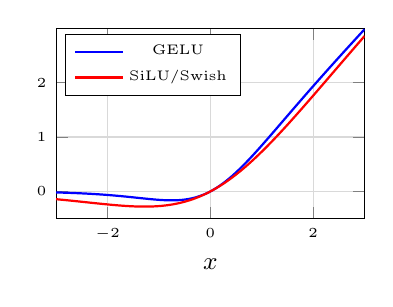
\begin{tikzpicture}
        \begin{axis}[width=5.5cm, height=4cm,
          xlabel={$x$}, ylabel={},
          xmin=-3, xmax=3, ymin=-0.5, ymax=3,
          grid=major, grid style={gray!30},
          legend pos=north west, legend style={font=\tiny},
          tick label style={font=\tiny},
          label style={font=\small},
          xtick={-2,0,2}, ytick={0,1,2}]
          \addplot[blue, thick, domain=-3:3, samples=80]
            {x * (1/(1+exp(-1.702*x)))};
          \addplot[red, thick, domain=-3:3, samples=80]
            {x * (1/(1+exp(-x)))};
          \legend{GELU, SiLU/Swish}
        \end{axis}
      \end{tikzpicture}
    \end{column}
  \end{columns}

  \vspace{0.3em}
  \begin{block}{Adoption}
    Used in LLaMA 1/2/3, Mistral, Gemma, PaLM. The gating mechanism provides more expressive non-linearity than a simple activation function.
  \end{block}
\end{frame}

% -----------------------------------------------------------------------
\begin{frame}{Parallel Attention + MLP}

  \textbf{Standard (sequential):} Attention and MLP run one after the other.

  \textbf{Parallel variant}~\cite{chowdhery2023palm}: Compute both from the same input, sum the results:
  \[
    x \leftarrow x + \text{Attn}(\text{Norm}(x)) + \text{MLP}(\text{Norm}(x))
  \]

  \vspace{0.3em}
  \begin{columns}[T]
    \begin{column}{0.48\textwidth}
      \centering
      \begin{tikzpicture}[
        box/.style={draw, rounded corners=3pt, minimum width=2.0cm, minimum height=0.5cm, font=\scriptsize, align=center},
        norm/.style={box, fill=yellow!20, draw=yellow!50!black},
        attn/.style={box, fill=orange!15},
        mlp/.style={box, fill=cyan!15},
        addcirc/.style={circle, draw=red!40, fill=red!8, inner sep=1.5pt, font=\tiny\bfseries, text=red!60!black},
        arr/.style={-{Stealth[length=3pt]}, thick, gray!70},
      ]
        \node[font=\scriptsize\bfseries] at (0, 4.6) {Sequential};
        \node[norm] (n1) at (0, 0.3) {Norm};
        \node[attn] (a1) at (0, 1.1) {Attn};
        \node[addcirc] (add1) at (0, 1.9) {$+$};
        \node[norm] (n2) at (0, 2.6) {Norm};
        \node[mlp] (m1) at (0, 3.4) {MLP};
        \node[addcirc] (add2) at (0, 4.2) {$+$};
        \draw[arr] (0,-0.1) -- (n1); \draw[arr] (n1) -- (a1); \draw[arr] (a1) -- (add1);
        \draw[arr] (add1) -- (n2); \draw[arr] (n2) -- (m1); \draw[arr] (m1) -- (add2);
        \draw[gray!50, thin, dashed, rounded corners=2pt] (-0.4,-0.0) -- (-1.3,0.0) -- (-1.3,1.9) -- (add1.west);
        \draw[gray!50, thin, dashed, rounded corners=2pt] (-0.4,2.1) -- (-1.3,2.1) -- (-1.3,4.2) -- (add2.west);
      \end{tikzpicture}

      {\scriptsize LLaMA, Mistral, DeepSeek, Qwen}
    \end{column}
    \begin{column}{0.48\textwidth}
      \centering
      \begin{tikzpicture}[
        box/.style={draw, rounded corners=3pt, minimum width=1.6cm, minimum height=0.5cm, font=\scriptsize, align=center},
        norm/.style={box, fill=yellow!20, draw=yellow!50!black, minimum width=2.0cm},
        attn/.style={box, fill=orange!15},
        mlp/.style={box, fill=cyan!15},
        addcirc/.style={circle, draw=red!40, fill=red!8, inner sep=1.5pt, font=\tiny\bfseries, text=red!60!black},
        arr/.style={-{Stealth[length=3pt]}, thick, gray!70},
      ]
        \node[font=\scriptsize\bfseries] at (0, 4.6) {Parallel};
        \node[norm] (n1) at (0, 0.3) {Norm};
        \node[attn] (a1) at (-1.0, 1.5) {Attn};
        \node[mlp] (m1) at (1.0, 1.5) {MLP};
        \node[addcirc] (add1) at (0, 2.7) {$+$};
        \draw[arr] (0,-0.1) -- (n1);
        \draw[arr] (n1.north) -- ++(-1.0, 0.4) -- (a1);
        \draw[arr] (n1.north) -- ++(1.0, 0.4) -- (m1);
        \draw[arr] (a1) -- (add1);
        \draw[arr] (m1) -- (add1);
        \draw[gray!50, thin, dashed, rounded corners=2pt] (-0.4,0.0) -- (-2.0,0.0) -- (-2.0,2.7) -- (add1.west);
      \end{tikzpicture}

      \vspace{0.7em}
      {\scriptsize GPT-J, PaLM}
    \end{column}
  \end{columns}

  \vspace{0.5em}
  \begin{columns}[T]
    \begin{column}{0.48\textwidth}
      \begin{block}{Advantage}
        Only one Norm per block. QKV and MLP input projections can be fused into one matmul. $\sim$15\% faster training.
      \end{block}
    \end{column}
    \begin{column}{0.48\textwidth}
      \begin{alertblock}{Trade-off}
        Small quality loss at $\le$8B scale. PaLM (540B) showed no degradation at large scale. Not the dominant choice today.
      \end{alertblock}
    \end{column}
  \end{columns}
\end{frame}

% -----------------------------------------------------------------------
\begin{frame}{Modern Decoder Block}

  Putting the improvements together: a modern decoder block (e.g.\ LLaMA~\cite{touvron2023llama}) vs.\ GPT-2.

  \vspace{0.3em}
  \begin{columns}[T]
    \begin{column}{0.48\textwidth}
      \centering\textbf{GPT-2 Block}
      \begin{align*}
        x &\leftarrow x + \text{Attn}(\text{LN}(x)) \\
        x &\leftarrow x + \text{MLP}(\text{LN}(x))
      \end{align*}

      \begin{itemize}
        \item LayerNorm (pre-norm)
        \item Multi-Head Attention
        \item GELU MLP ($d \to 4d \to d$)
        \item Learned absolute positions
        \item Biases in linear layers
      \end{itemize}
    \end{column}
    \begin{column}{0.48\textwidth}
      \centering\textbf{LLaMA / Gemma Block}
      \begin{align*}
        x &\leftarrow x + \text{GQA}(\text{RMSNorm}(x)) \\
        x &\leftarrow x + \text{SwiGLU}(\text{RMSNorm}(x))
      \end{align*}

      \begin{itemize}
        \item RMSNorm (pre-norm or Peri-LN)
        \item GQA + RoPE (+ optional QK-norm)
        \item SwiGLU MLP ($d \to \tfrac{8}{3}d \to d$)
        \item RoPE (relative positions)
        \item No biases anywhere
      \end{itemize}
    \end{column}
  \end{columns}

  \vspace{0.5em}
  \begin{alertblock}{Same skeleton, different components}
    The residual stream with pre-norm attention and MLP remains unchanged.
    Every sub-component has been upgraded for better quality and efficiency.
  \end{alertblock}
\end{frame}

\subsection{Attention Sinks and Mitigations}

% -----------------------------------------------------------------------
\begin{frame}{Attention Sinks~\cite{xiao2024streamingllm}}

  \begin{columns}[T]
    \begin{column}{0.55\textwidth}
      \textbf{Observation:} LLMs assign disproportionate attention to the BOS / first token,
      even though it carries no special semantic information. This occurs across nearly all heads and layers.

      \vspace{0.3em}
      \textbf{Why?} Softmax forces $\sum_j \alpha_j = 1$.
      When a head has nothing useful to retrieve, it cannot output zero.
      It dumps the surplus mass on the first token (always visible in causal attention).

      \vspace{0.3em}
      \textbf{Consequences:}
      \begin{itemize}
        \item \textbf{KV-cache eviction breaks:} Evicting the sink token's KV pair from a sliding window causes perplexity to explode
        \item \textbf{Massive activations:} Sink tokens develop hidden-state values $\sim\!100{,}000\times$ larger than normal, breaking quantization
        \item \textbf{Wasted capacity:} Many heads spend computation on a semantically meaningless token
      \end{itemize}
    \end{column}
    \begin{column}{0.43\textwidth}
      \centering
      \begin{tikzpicture}[scale=0.85,
          tok/.style={draw=gray!50, rounded corners=2pt, minimum height=0.35cm,
                      minimum width=0.6cm, inner sep=2pt, font=\tiny},
          arr/.style={-{Stealth[length=2.5pt]}, thick},
        ]
        % Tokens
        \node[tok, fill=red!25, line width=0.8pt, draw=red!50] (bos) at (0, 3.0) {BOS};
        \node[tok, fill=gray!10] (t1) at (0.9, 3.0) {The};
        \node[tok, fill=gray!10] (t2) at (1.8, 3.0) {cat};
        \node[tok, fill=gray!10] (t3) at (2.7, 3.0) {sat};

        % Query token
        \node[tok, fill=blue!15] (q) at (1.35, 1.2) {query: sat};

        % Attention arrows (thickness = weight)
        \draw[arr, red!60, line width=2.5pt] (q) -- (bos) node[midway, left, font=\tiny, red!60!black] {47\%};
        \draw[arr, gray!50, line width=0.4pt] (q) -- (t1) node[midway, right, font=\tiny, gray] {8\%};
        \draw[arr, gray!50, line width=0.8pt] (q) -- (t2) node[pos=0.6, right, font=\tiny, gray] {18\%};
        \draw[arr, gray!50, line width=1.2pt] (q) -- (t3);

        \node[font=\scriptsize, gray, align=center] at (1.35, 0.4) {Attention mass ``dumped''\\on first token};
      \end{tikzpicture}

      \vspace{0.3em}
      \begin{block}{\small StreamingLLM fix}
        Always keep first 1--4 tokens in KV-cache alongside the sliding window.
        Simple workaround, no retraining.
      \end{block}
    \end{column}
  \end{columns}
\end{frame}

% -----------------------------------------------------------------------
\begin{frame}{Mitigating Attention Sinks}

  The root cause is that softmax cannot express ``attend to nothing.'' Several architectural fixes exist:

  \vspace{0.5em}
  \begin{description}[labelwidth=2.8cm, leftmargin=3.0cm]
    \item[Gated attention] Per-head sigmoid gate after attention output (next slide). The gate can scale the output to near zero, eliminating the need for a sink.
    \item[Learned sink bias] Add one learnable scalar $b_i$ per head to the softmax denominator:
      \[
        \alpha_j = \frac{\exp(s_j)}{\exp(b_i) + \sum_{j'} \exp(s_{j'})}
      \]
      This gives the head a learnable ``virtual zero token.'' Used in OpenAI's open-source model.
    \item[Softmax$_1$] Replace softmax denominator $\sum_j \exp(s_j)$ with $1 + \sum_j \exp(s_j)$.
      Allows total attention weight $< 1$ without any learned parameters.
  \end{description}

  \vspace{0.3em}
  \begin{alertblock}{Practical impact}
    Attention sinks also cause massive activation outliers ($100{,}000\times$ normal), which severely degrade INT8/INT4 quantization.
    Mitigating sinks directly improves quantization quality.
  \end{alertblock}
\end{frame}

% -----------------------------------------------------------------------
\begin{frame}{Gated Attention~\cite{qiu2025gatedattention}}

  Add a learned, per-head sigmoid gate \emph{after} the softmax attention output:
  \[
    \text{head}_i = \sigma\!\bigl(g_i(q)\bigr) \cdot \text{softmax}\!\left(\frac{Q_i K_i^\top}{\sqrt{d_k}}\right) V_i
  \]
  where $g_i(q) \in \mathbb{R}$ is a scalar gate depending on the query.

  \vspace{0.3em}
  \begin{columns}[T]
    \begin{column}{0.48\textwidth}
      \textbf{Effects:}
      \begin{itemize}
        \item Sink attention drops from $\sim$47\% to $\sim$5\%
        \item Massive activations disappear
        \item Improved training stability and tolerance for higher learning rates
        \item Adds non-linearity that breaks the low-rank bottleneck of softmax attention
      \end{itemize}

      \vspace{0.3em}
      \begin{alertblock}{\small Status}
        NeurIPS 2025 best paper.
        Adopted by Qwen3-Next/3.5.
        Very promising but not yet widely deployed beyond Qwen.
      \end{alertblock}
    \end{column}
    \begin{column}{0.48\textwidth}
      \centering
      \begin{tikzpicture}[
        box/.style={draw, rounded corners=3pt, minimum width=2.0cm, minimum height=0.5cm, font=\scriptsize, align=center},
        arr/.style={-{Stealth[length=3pt]}, thick, gray!70},
        mul/.style={circle, draw=blue!50, fill=blue!10, inner sep=1.5pt, font=\tiny\bfseries},
      ]
        \node[box, fill=gray!10] (qkv) at (0, 4.0) {$Q_i, K_i, V_i$};
        \node[box, fill=orange!15] (attn) at (-0.8, 2.8) {$\text{softmax}(\frac{QK^\top}{\sqrt{d}})V$};
        \node[box, fill=green!15] (gate) at (1.4, 2.8) {$\sigma(g_i(q))$};
        \node[mul] (m) at (0, 1.6) {$\times$};
        \node[box, fill=blue!10] (out) at (0, 0.5) {$\text{head}_i$};
        \draw[arr] (qkv) -- (attn);
        \draw[arr] (qkv) -- (gate);
        \draw[arr] (attn) -- (m);
        \draw[arr] (gate) -- (m);
        \draw[arr] (m) -- (out);
      \end{tikzpicture}

      \vspace{0.3em}
      {\footnotesize The gate $g_i(q)$ is a simple linear projection of the query. One scalar per head, negligible parameter overhead.}
    \end{column}
  \end{columns}
\end{frame}

